\chapter{Metodologia}
\label{chap:metodologia}

Este capítulo apresenta a metodologia de implementação e o plano de avaliação da arquitetura proposta. A Seção~\ref{sec:visao_geral_arquitetura_edgar} apresenta a topologia do sistema e sua divisão em fluxos operacionais. A Seção~\ref{sec:definicao_componentes_tecnologicos} detalha as tecnologias adotadas para atender aos requisitos da arquitetura. Nas seções subsequentes, são mapeadas as etapas de engenharia de dados do fluxo assíncrono de ingestão, as fases de inferência do fluxo síncrono de recuperação e, por fim, o protocolo de validação experimental.

\section{Visão geral da arquitetura EDGAR}
\label{sec:visao_geral_arquitetura_edgar}

A arquitetura EDGAR deve operar como um \textit{pipeline} de processamento de dados projetado para desacoplar as etapas de curadoria documental da interação em tempo real com o usuário. Operacionalmente, o sistema não exige treinamento adicional (\textit{training-free}), funcionando por meio da orquestração de modelos de visão, extração e linguagem em uma topologia modular. 

Para mitigar a latência durante as consultas, o sistema divide-se logicamente em dois fluxos operacionais:
\begin{enumerate}
    \item \textbf{Fluxo assíncrono de ingestão e indexação (\textit{offline}):} Concentra a carga computacional pesada. É responsável por receber o documento PDF, realizar a segmentação visual de seus componentes, gerar transcrições e descrições semânticas, e armazenar as representações vetoriais juntamente com seus metadados espaciais.
    \item \textbf{Fluxo síncrono de recuperação e geração (\textit{online}):} Atua estritamente sob demanda. Acionado exclusivamente quando uma consulta é realizada, esse fluxo responsabiliza-se por vetorizar a entrada do usuário, recuperar as evidências em granularidade fina, formatar o contexto e executar a inferência no modelo gerador.
\end{enumerate}

A interação com o usuário ocorre por meio da aplicação cliente LuminIA Reader. No contexto desta arquitetura, ela é responsável pelo envio de arquivos, pela submissão de consultas e pela renderização das respostas e das coordenadas espaciais retornadas pelo fluxo síncrono. Como se trata de um componente instrumental de suporte à validação e não do escopo científico principal desta pesquisa, seus detalhes de engenharia de \textit{software}, camadas arquiteturais e fluxos de estados internos encontram-se documentados no Apêndice~\ref{ap:luminia-reader}. A Figura~\ref{fig:pipeline_edgar} ilustra a topologia citada, evidenciando a integração entre os fluxos operacionais da arquitetura e a aplicação cliente.

\begin{figure}[ht]
\centering
\begin{minipage}{\textwidth}
\caption{Visão geral do funcionamento da arquitetura EDGAR.}
\label{fig:pipeline_edgar}
\vspace{0.2cm}
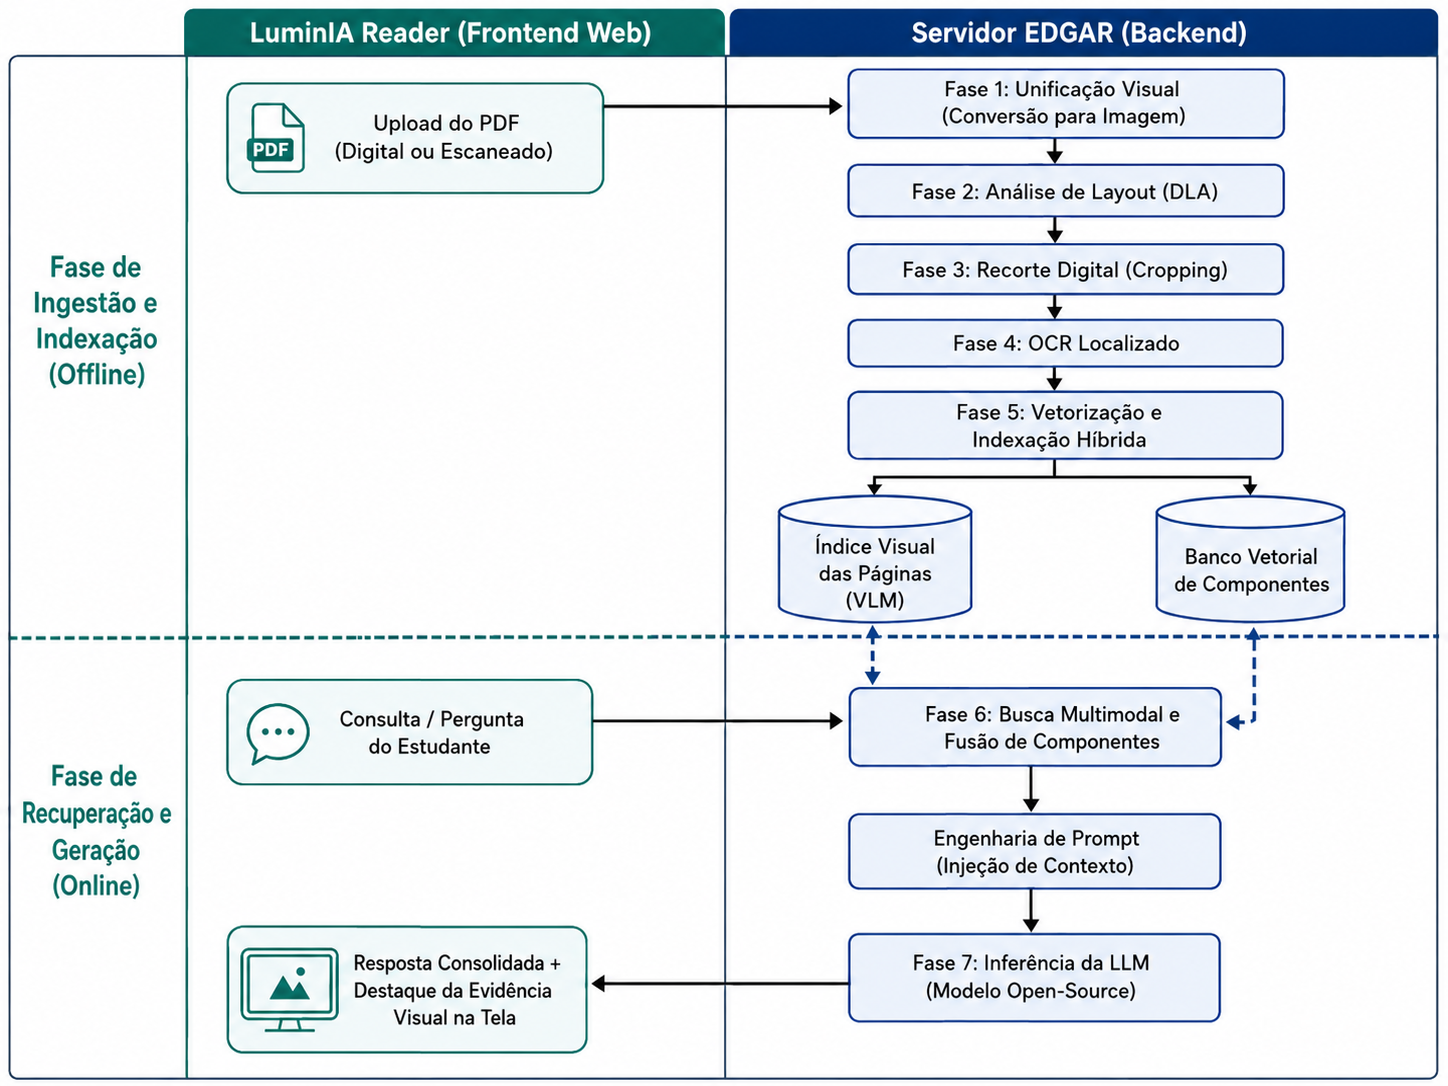
\includegraphics[width=\textwidth]{figuras/pipeline_edgar}
\vspace{0.1cm}
\\ {\footnotesize Fonte: Elaborado pelo autor.}
\end{minipage}
\end{figure}

\section{Definição dos componentes tecnológicos}
\label{sec:definicao_componentes_tecnologicos}

A arquitetura exige ferramentas capazes de atuar sobre matrizes de imagens, extração de \textit{strings}, inferência de redes neurais e cálculos de similaridade vetorial. A Tabela~\ref{tab:componentes-tecnologicos} mapeia as tecnologias de código aberto selecionadas para compor as fases de processamento do sistema e sua camada de aplicação cliente.

\begin{table}[H]
\centering
\caption{Componentes tecnológicos definidos para a arquitetura do presente trabalho e sua camada de aplicação cliente.}
\label{tab:componentes-tecnologicos}

\renewcommand{\arraystretch}{1.35}
\begin{tabularx}{\textwidth}{|p{3.5cm}|p{4.0cm}|X|}
\hline
\textbf{Módulo} & \textbf{Tecnologia definida} & \textbf{Função na arquitetura} \\
\hline

Conversão de PDF para imagem 
& PyMuPDF 
& Renderizar páginas PDF como imagens padronizadas para análise visual. \\
\hline

Análise de layout de documentos 
& DocLayout-YOLO 
& Detectar regiões estruturais da página e gerar \textit{bounding boxes}. \\
\hline

Isolamento geométrico 
& OpenCV 
& Recortar componentes visuais a partir das coordenadas detectadas. \\
\hline

Extração textual localizada 
& PyMuPDF / Tesseract OCR 
& Extrair texto de componentes digitais ou escaneados. \\
\hline

Descrição visual de componentes
& Qwen2.5-VL-7B-Instruct
& Gerar descrições textuais estruturadas de elementos visuais recortados. \\
\hline

Vetorização textual 
& BGE-M3 via Sentence Transformers 
& Gerar vetores semânticos dos textos extraídos e descrições visuais. \\
\hline

Banco de dados vetorial 
& Qdrant 
& Armazenar \textit{embeddings} e metadados dos componentes documentais. \\
\hline

Modelo de linguagem gerador 
& Qwen2.5-7B-Instruct 
& Gerar respostas a partir das evidências recuperadas. \\
\hline

Interface web 
& Vue.js / PDF.js 
& Implementar a aplicação cliente LuminIA Reader. \\
\hline

\end{tabularx}

\legend{Fonte: Elaborado pelo autor.}
\end{table}

\subsection{Justificativa operacional das tecnologias adotadas}

A adoção das ferramentas listadas na Tabela~\ref{tab:componentes-tecnologicos} baseia-se na capacidade de cada tecnologia em atender aos requisitos de processamento de dados do \textit{pipeline}, garantindo a interoperabilidade entre as etapas visuais e semânticas.

\begin{itemize}

    \item \textbf{PyMuPDF:} Adotado para a renderização inicial das páginas (Fase 1) e para a extração primária de texto (Fase 4). Operacionalmente, sua escolha justifica-se pela capacidade de expor coordenadas espaciais precisas do texto digital, permitindo a correlação matemática exata entre os recortes da imagem rasterizada e as \textit{strings} subjacentes do arquivo PDF.

    \item \textbf{DocLayout-YOLO:} Selecionado para a etapa de detecção geométrica (Fase 2). Ao contrário de abordagens multimodais pesadas, a escolha do YOLO atende ao requisito de alta velocidade de inferência na delimitação de componentes (\textit{bounding boxes}). A independência de uma etapa prévia de OCR torna-o ideal para processar assincronamente grandes volumes de páginas renderizadas.

    \item \textbf{OpenCV:} Utilizado como motor de manipulação matricial (Fase 3). Sua função é receber as coordenadas cartesianas geradas pelo modelo YOLO e realizar recortes lógicos sobre as imagens base. A biblioteca atende ao requisito de preparar os artefatos isolados sem perda de resolução, viabilizando o processamento isolado pelas redes neurais subsequentes.

    \item \textbf{Tesseract OCR:} Implementado como mecanismo de contingência (\textit{fallback}) na extração de texto (Fase 4). Sua adoção operacional visa garantir a captura de texto em documentos escaneados ou em componentes visuais complexos que não possuem camada de texto acessível via PyMuPDF.
    
    \item \textbf{Qwen2.5-VL-7B-Instruct:} Integrado ao \textit{pipeline} assíncrono (Fase 5) para atuar exclusivamente sobre recortes visuais cujas relações semânticas são invisíveis a extratores tradicionais. A escolha desse modelo específico fundamenta-se em sua capacidade instrucional de traduzir relações espaciais de tabelas, eixos de gráficos e arranjos de fórmulas matemáticas em texto estruturado formatado nativamente para indexação.

    \item \textbf{BGE-M3 (Sentence Transformers):} Designado como o modelo unificado de vetorização (Fase 6 e Fase 7). Sua implementação atende à exigência de criar representações densas multilíngues com suporte a comprimentos variados de entrada, garantindo que fragmentos textuais curtos, descrições extensas geradas por VLM e perguntas diretas do usuário habitem o mesmo espaço vetorial de busca.

    \item \textbf{Qdrant:} Adotado como infraestrutura de armazenamento e busca vetorial. A justificativa técnica para seu uso reside em seu suporte otimizado a consultas híbridas. O EDGAR depende nativamente da capacidade de anexar metadados em formato JSON (\textit{payloads}) aos \textit{embeddings}, recurso que o Qdrant oferece em tempo real, permitindo cruzar a similaridade do cosseno com restrições por identificador de documento e classe de componente.

   \item \textbf{Vue.js e PDF.js:} Definidos para orquestrar a camada de apresentação do LuminIA Reader. A escolha combinada atende ao requisito de mapeamento reativo: enquanto o Vue.js manipula o estado do painel de respostas via chamadas de API, o PDF.js permite renderizar o documento no navegador e transpor as coordenadas geométricas retornadas pelo EDGAR diretamente sobre o canvas visual, destacando a evidência correta para o estudante.

\end{itemize}

\section{Fluxo assíncrono de ingestão e indexação}
\label{sec:fluxo_assincrono_ingestao_indexacao}

O fluxo assíncrono de ingestão e indexação (\textit{offline}) opera como o primeiro estágio do \textit{pipeline} de dados da arquitetura. Ele é encarregado de processar os documentos didáticos submetidos pela aplicação cliente e transformá-los em uma base de conhecimento multimodal, estruturada em unidades de granularidade fina. A execução em segundo plano visa garantir que as etapas computacionalmente mais custosas, como inferência visual e geração de \textit{embeddings}, sejam finalizadas antes de qualquer interação do usuário.

Esse fluxo é arquitetado em seis fases sequenciais, formatadas sob o paradigma de engenharia de dados, nas quais a saída de um módulo atua estritamente como a entrada do módulo subsequente.

\subsection{Fase 1: Unificação visual e normalização de entrada}
\label{subsec:fase1_unificacao_visual}

\begin{itemize}
    \item \textbf{Entrada:} Arquivo PDF bruto, contendo páginas que podem mesclar camadas de texto digital e regiões escaneadas.
    \item \textbf{Processamento:} O arquivo é processado pelo módulo PyMuPDF, que realiza a renderização e padronização visual de todas as páginas. A conversão é fixada operacionalmente na resolução de 300 DPI, valor mapeado como o ponto de equilíbrio ótimo entre a preservação de detalhes geométricos essenciais e o custo computacional de processamento de matrizes.
    \item \textbf{Saída:} Uma coleção de imagens rasterizadas (uma por página), indexadas pelos metadados fundamentais do documento original (identificador do arquivo, número da página e dimensões de largura e altura).
\end{itemize}

\subsection{Fase 2: Análise de layout de documentos (DLA)}
\label{subsec:fase2_analise_layout}

\begin{itemize}
    \item \textbf{Entrada:} Imagens rasterizadas geradas na Fase 1.
    \item \textbf{Processamento:} As matrizes visuais são submetidas à inferência do modelo DocLayout-YOLO. A rede neural realiza a detecção estritamente visual das topologias da página, classificando os componentes lógicos de acordo com suas categorias estruturais (como \textit{plain\_text}, \textit{title}, \textit{table}, \textit{figure}, \textit{isolate\_formula}, entre outros).
    \item \textbf{Saída:} Um conjunto de artefatos lógicos contendo o rótulo da classe detectada, o índice estatístico de confiança da predição e, criticamente, as coordenadas espaciais que delimitam o elemento na página (\textit{bounding boxes} mapeadas nos eixos cartesianos X e Y).
\end{itemize}

\subsection{Fase 3: Isolamento geométrico de componentes (\textit{cropping})}
\label{subsec:fase3_isolamento_geometrico}

\begin{itemize}
    \item \textbf{Entrada:} Matrizes de imagem (Fase 1) mapeadas contra as coordenadas geométricas delimitadas (\textit{bounding boxes} da Fase 2).
    \item \textbf{Processamento:} O OpenCV é acionado para aplicar operações de recorte matricial direto. Nesta etapa, componentes avaliados como ruído estrutural (artefatos classificados como \textit{abandon}, abrangendo cabeçalhos e numerações de página) são descartados. Simultaneamente, componentes lógicos de legenda (\texttt{figure\_caption} e \texttt{table\_caption}) são preservados e submetidos a um cálculo de proximidade espacial. O sistema mede a distância entre centroides para vincular geometricamente cada legenda à figura ou tabela correspondente mais próxima na mesma página.
    \item \textbf{Saída:} Imagens menores e isoladas correspondentes a cada componente válido da página. Os artefatos de legenda recebem a injeção de um metadado estrutural adicional no seu \textit{payload}, denominado \texttt{componente\_pai}, preservando a hierarquia visual para as fases subsequentes de extração, indexação e engenharia de contexto.
\end{itemize}

\subsection{Fase 4: Extração textual localizada (OCR seletivo)}
\label{subsec:fase4_ocr_localizado}

\begin{itemize}
    \item \textbf{Entrada:} Coordenadas dos componentes lógicos e seus respectivos recortes geométricos.
    \item \textbf{Processamento:} O sistema aplica uma estratégia híbrida de extração de caracteres. Primeiramente, utiliza o PyMuPDF para mapear as coordenadas do componente (\textit{bounding box}) contra a camada de texto nativa do arquivo digital, extraindo as \textit{strings} exatas daquela região. Em casos de falha, de arquivos escaneados ou de áreas gráficas específicas, o sistema executa a contingência (\textit{fallback}), disparando o motor Tesseract OCR diretamente sobre a matriz recortada na Fase 3.
    \item \textbf{Saída:} Uma \textit{string} de texto delimitada, associada estritamente aos contornos daquele componente específico, para garantir que parágrafos de colunas diferentes não sejam sobrepostos indevidamente.
\end{itemize}

\subsection{Fase 5: Descrição visual de componentes}
\label{subsec:fase5_descricao_visual}

\begin{itemize}
    \item \textbf{Entrada:} Recortes visuais puramente não-textuais (como componentes previamente classificados em \textit{figure}, \textit{table} ou \textit{isolate\_formula}).
    \item \textbf{Processamento:} O modelo gerador Qwen2.5-VL-7B-Instruct realiza a análise do recorte visual. A inferência é configurada para representar informações que extrapolam a capacidade de extração do OCR, traduzindo propriedades visuais, como agrupamentos lógicos em tabelas, a topologia de um diagrama ou sintaxe de equações matemáticas, em descrições textuais de caráter analítico.
    \item \textbf{Saída:} Uma \textit{string} complementar de descrição estruturada contendo o tipo do elemento, a síntese do seu conteúdo e as relações espaciais observadas, atuando como o enriquecimento semântico do componente.
\end{itemize}

\subsection{Fase 6: Vetorização e indexação multimodal híbrida}
\label{subsec:fase6_indexacao_hibrida}

\begin{itemize}
    \item \textbf{Entrada:} A totalidade dos fragmentos processados, compreendendo as transcrições de texto da Fase 4, as descrições visuais geradas na Fase 5 e os metadados acumulados.
    \item \textbf{Processamento:} Os artefatos textuais são processados pelo modelo multilíngue BGE-M3 (via biblioteca Sentence Transformers), que os projeta matematicamente em \textit{embeddings} de alta dimensionalidade. Simultaneamente, o EDGAR estrutura um pacote JSON (\textit{payload}) agregando os metadados espaciais de origem.
    \item \textbf{Saída:} Indexação final no banco de dados vetorial Qdrant. Cada registro armazenado passa a conter o \textit{embedding} semântico atrelado a um \textit{payload} obrigatório com os seguintes campos: identificador do documento (\texttt{doc\_id}), número da folha (\texttt{pagina}), rótulo estrutural (\texttt{classe}), coordenadas X/Y (\texttt{bbox}), texto transcrito (\texttt{texto\_extraido}), texto descritivo (\texttt{descricao\_visual}) e referência física do recorte (\texttt{crop\_ref}).
\end{itemize}

\section{Fluxo síncrono de recuperação e geração}
\label{sec:fluxo_sincrono_recuperacao_geracao}

O fluxo síncrono de recuperação e geração (\textit{online}) atua como o motor de inferência em tempo real da arquitetura. Operando estritamente sobre a base vetorial populada durante a etapa de ingestão, este fluxo é projetado para minimizar a latência computacional. Suas operações restringem-se à vetorização da consulta, à busca matemática por similaridade e à orquestração do \textit{prompt} para o modelo de linguagem principal. O processo é estruturado em duas fases analíticas, resultando no empacotamento dos dados para a camada de apresentação.

\subsection{Fase 7: Recuperação semântica e associação de evidências}
\label{subsec:fase7_recuperacao_evidencias}

\begin{itemize}
    \item \textbf{Entrada:} Pergunta em linguagem natural submetida pelo estudante via aplicação cliente.
    \item \textbf{Processamento:} A consulta é codificada pelo modelo BGE-M3, garantindo paridade dimensional com o espaço vetorial do banco de dados. O vetor resultante é utilizado para executar uma busca por similaridade geométrica (cosseno) no Qdrant, recuperando os componentes mais próximos (\textit{Top-K}). A operação resgata o \textit{payload} completo de cada registro, recompondo a evidência por meio do cruzamento entre sua classe estrutural, texto nativo e descrição visual gerada previamente.
    \item \textbf{Saída:} Um subconjunto ordenado de componentes de alta relevância, contendo a síntese semântica e as coordenadas espaciais necessárias para a sustentação da resposta.
\end{itemize}

\subsection{Fase 8: Engenharia de contexto e inferência}
\label{subsec:fase8_engenharia_contexto}

\begin{itemize}
    \item \textbf{Entrada:} A consulta original do usuário e o subconjunto de evidências estruturadas recuperadas na Fase 7.
    \item \textbf{Processamento:} O módulo de engenharia de contexto organiza as evidências recuperadas na Fase 7 em um \textit{prompt} de instrução fechada estruturado em três seções distintas. A primeira seção, denominada \texttt{[INSTRUÇÃO]}, direciona o modelo gerador a basear sua resposta exclusivamente nos fragmentos fornecidos, inibindo a produção de conteúdo não fundamentado nas evidências. A segunda seção, \texttt{[EVIDÊNCIAS]}, apresenta os componentes recuperados em ordem decrescente de pontuação de similaridade, cada um acompanhado de sua classe estrutural, número de página e identificador de documento. Para componentes textuais (\texttt{plain\_text}, \texttt{title}), é injetado o campo \texttt{texto\_extraido}; para componentes visuais (\texttt{table}, \texttt{figure}, \texttt{isolate\_formula}), é injetado o campo \texttt{descricao\_visual} gerado na Fase 5. A terceira seção, \texttt{[PERGUNTA]}, apresenta a consulta original do usuário sem modificações. Para preservar o desempenho de latência (\textit{time-to-first-token}), as matrizes de imagem dos recortes visuais não são transmitidas ao modelo gerador; a inferência atua exclusivamente sobre a representação textual enriquecida produzida na Fase 5. A parametrização da chamada ao modelo condiciona a geração à presença obrigatória de citação à evidência utilizada, viabilizando a rastreabilidade da resposta ao componente documental de origem.
    \item \textbf{Saída:} Um objeto JSON final contendo a resposta articulada em linguagem natural e a relação explícita dos componentes utilizados como fontes, com seus respectivos identificadores de documento, página e metadados geométricos.
\end{itemize}

\subsection{Interação com a aplicação cliente e visualização de evidências}
\label{subsec:interacao_aplicacao_cliente}

A etapa final do fluxo síncrono consiste no retorno de um \textit{payload} JSON ao LuminIA Reader. Ao receber esse pacote de dados, os controladores da interface (Vue.js) atualizam o estado do painel de respostas e encaminham as coordenadas espaciais (\textit{bounding boxes}) para o mecanismo de renderização do PDF.js. Esse processo converte as posições cartesianas em marcações visuais sobrepostas à página exibida no navegador (\textit{canvas}), permitindo que o estudante identifique exatamente qual tabela, figura ou parágrafo fundamentou a resposta gerada pelo sistema.

A sequência de interações e a troca de mensagens ao longo desse ciclo são apresentadas na Figura~\ref{fig:interacao_fluxo_online}, que ilustra a requisição originada na aplicação cliente, sua passagem pelo banco vetorial e pelo modelo gerador, e o retorno da resposta acompanhada de suas referências espaciais.


\begin{figure}[ht]
\centering
\begin{minipage}{\textwidth}
\caption{Diagrama de sequência do fluxo síncrono de recuperação e geração da arquitetura.}
\label{fig:interacao_fluxo_online}
\vspace{0.2cm}
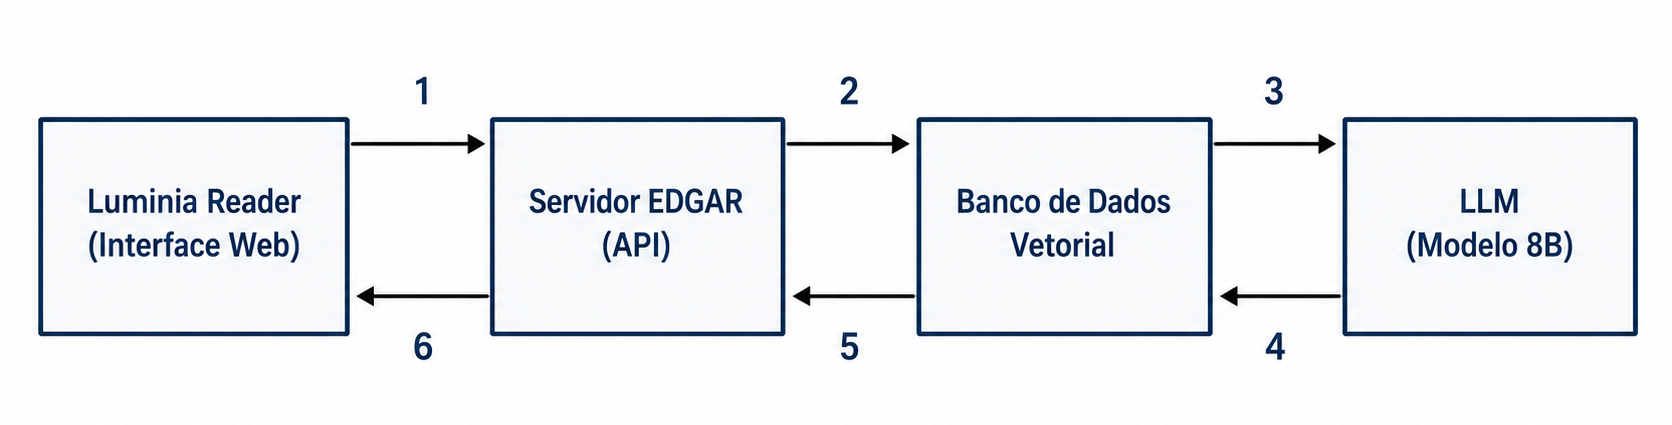
\includegraphics[width=\textwidth]{figuras/interacao_fluxo_online}
\vspace{0.1cm}
\\ {\footnotesize Fonte: Elaborado pelo autor.}
\end{minipage}
\end{figure}

\section{Plano de avaliação experimental}
\label{sec:plano_avaliacao_experimental}

O plano de avaliação experimental tem como objetivo validar, de forma quantitativa e qualitativa, a eficácia da arquitetura proposta no presente trabalho. O protocolo foi concebido para isolar o impacto da granularidade fina na mitigação de ruído estrutural e de alucinações. Para assegurar a reprodutibilidade e o rigor científico da análise, a validação está estruturada em quatro dimensões: infraestrutura experimental, \textit{dataset} de validação, cenários de controle (\textit{baselines}) e métricas de desempenho.

\subsection{Ambiente de execução e infraestrutura computacional}
\label{subsec:ambiente_execucao}

Para refletir um cenário de implementação realista e isolar a carga computacional, o protocolo de testes adotará a seguinte separação de ambientes:
\begin{itemize}
    \item \textbf{Arquitetura EDGAR:} Operará em infraestrutura de nuvem baseada em Linux e provisionada com contêineres Docker. Esse ambiente concentrará a aceleração via GPU necessária para as inferências do modelo de visão (DocLayout-YOLO), do gerador multimodal (Qwen2.5-VL), do vetorizador (BGE-M3) e do gerador textual (Qwen2.5-7B). Técnicas de quantização poderão ser aplicadas aos modelos de linguagem da classe 7B--8B para viabilizar a execução em restrições de memória de vídeo (VRAM).
    \item \textbf{Aplicação cliente LuminIA Reader:} Será executada em ambiente de desenvolvimento convencional. No escopo do protocolo experimental, sua função restringe-se a consumir os serviços da arquitetura: disparar os gatilhos de tempo para cálculo de latência de rede, submeter as perguntas do \textit{dataset} e atestar a correta renderização visual das \textit{bounding boxes} retornadas.
\end{itemize}

\subsection{Conjunto de documentos e consultas (\textit{Dataset} de avaliação)}
\label{subsec:conjunto_documentos_perguntas}

A avaliação não utilizará \textit{datasets} genéricos, mas um conjunto de dados desenvolvido especificamente para o domínio educacional, composto por dois elementos principais:

\begin{enumerate}
\item \textbf{Base Documental:} Uma amostra curada de materiais didáticos reais em formato PDF, com foco em disciplinas de ciências exatas. A escolha desse domínio deve-se à sua complexidade e à diversidade de elementos visuais presentes nos documentos, proporcionando um cenário desafiador para a avaliação do sistema. O conjunto incluirá páginas com texto denso, tabelas de dados, diagramas relacionais e fórmulas matemáticas.

\item \textbf{Consultas de Validação:} Um repositório de perguntas que simulam dúvidas reais de estudantes. Para fins de avaliação, cada pergunta será associada a um gabarito de referência previamente definido. Esse gabarito especificará a página, a classe geométrica, a transcrição textual ou a informação visual que deverá ser recuperada pelo EDGAR para que a resposta seja considerada correta.

\end{enumerate}


\subsection{Configurações comparativas (\textit{Baselines})}
\label{subsec:configuracoes_comparativas}

Para mensurar o ganho de desempenho isolado de cada componente metodológico da arquitetura, a avaliação submeterá o mesmo \textit{dataset} a quatro configurações de recuperação distintas. O objetivo é estabelecer linhas de base (\textit{baselines}) para contrastar o paradigma de \textit{chunking} linear com o particionamento visual de granularidade fina. A Tabela~\ref{tab:configuracoes_comparativas} consolida essas configurações.

\begin{table}[H]
\centering
\caption{Configurações comparativas previstas para a avaliação experimental.}
\label{tab:configuracoes_comparativas}

\begin{minipage}{\textwidth}
\renewcommand{\arraystretch}{1.3}
\begin{tabularx}{\textwidth}{|p{3.2cm}|p{5.0cm}|X|}
\hline
\textbf{Configuração} & \textbf{Descrição} & \textbf{Objetivo da comparação} \\
\hline

RAG textual tradicional
& Extração textual do PDF seguida de segmentação em blocos de tamanho fixo.
& Verificar o desempenho de uma abordagem baseada apenas em texto linearizado. \\
\hline

RAG por página
& Indexação e recuperação considerando páginas inteiras como unidades de contexto.
& Avaliar o impacto do uso de contextos mais amplos e potencialmente mais ruidosos. \\
\hline

EDGAR sem descrição visual
& Recuperação por componentes com texto extraído, metadados e recortes visuais, mas sem descrição visual automática.
& Isolar o impacto da etapa de descrição visual sobre a recuperação e a geração. \\
\hline

EDGAR completo
& Recuperação por componentes com texto extraído, descrição visual, recorte visual e metadados geométricos.
& Avaliar a arquitetura proposta em sua configuração completa de granularidade fina. \\
\hline

\end{tabularx}

\par\vspace{0.1cm}
{\raggedright\footnotesize Fonte: Elaborado pelo autor.\par}
\end{minipage}
\end{table}

\subsection{Métricas e protocolo de avaliação}
\label{subsec:metricas_protocolo}

Os resultados de cada configuração comparativa serão parametrizados em três eixos de medição empírica:
\begin{itemize}
    \item \textbf{Desempenho Computacional:} Mensuração de custo de máquina e tempo. Inclui o tempo absoluto de processamento do fluxo \textit{offline} (por página e por documento) e a métrica de latência de ponta a ponta ($L_{p2p}$) no fluxo \textit{online}, calculada do despacho da \textit{string} de consulta até o retorno completo do \textit{payload} JSON.
    \item \textbf{Qualidade de Recuperação (Rastreabilidade):} Avaliada pelo cruzamento dos artefatos recuperados contra o \textit{ground-truth}. Utilizará a métrica \textit{Context Precision} e \textit{Recall@k} para atestar se a arquitetura priorizou geometricamente as evidências corretas no ranqueamento vetorial.
    \item \textbf{Qualidade de Geração (Semântica):} As inferências do modelo gerador serão avaliadas por meio das métricas propostas pelo \textit{framework} RAGAS \citeb{es2024ragas}: \textit{Faithfulness} (fidelidade contextual), que quantifica a proporção de afirmações da resposta que podem ser diretamente atribuídas às evidências fornecidas no contexto, constituindo uma medida objetiva da ausência de alucinações extrínsecas; e \textit{Answer Relevance} (relevância da resposta), que avalia o grau de aderência da resposta à pergunta submetida, penalizando respostas que, embora factuais, desviem do foco da consulta. Ambas as métricas são calculadas de forma automatizada a partir da tripla (pergunta, evidências recuperadas e resposta gerada), conforme especificado em \citeonline{es2024ragas}.

\end{itemize}

A Tabela~\ref{tab:matriz_experimentos} mapeia essas dimensões contra seus respectivos módulos e critérios de avaliação.

\begin{table}[H]
\centering
\caption{Matriz de componentes e métricas previstas para a avaliação experimental.}
\label{tab:matriz_experimentos}

\renewcommand{\arraystretch}{1.3}
\begin{tabularx}{\textwidth}{|p{3.6cm}|p{4.2cm}|X|}
\hline
\textbf{Dimensão avaliada} & \textbf{Componente / aspecto} & \textbf{Métrica ou critério de avaliação} \\
\hline

Infraestrutura
& Servidor em nuvem com Docker e GPU
& Uso de memória, compatibilidade de execução e estabilidade do ambiente. \\
\hline

Fluxo assíncrono
& Ingestão, análise de layout, OCR e descrição visual
& Tempo de processamento por documento e por página. \\
\hline

Descrição visual
& Qwen2.5-VL-7B-Instruct
& Tempo de geração das descrições e utilidade semântica para recuperação. \\
\hline

Recuperação vetorial
& BGE-M3 e Qdrant
& \textit{Context Precision}, Recall@k e posição do primeiro componente correto. \\
\hline

Geração da resposta
& Qwen2.5-7B-Instruct
& \textit{Faithfulness}, \textit{Answer Relevance}, taxa de geração de tokens e aderência às evidências. \\
\hline

Fluxo síncrono
& Consulta cliente-servidor
& Latência de ponta a ponta ($L_{p2p}$), tempo de recuperação e tempo de inferência. \\
\hline

Rastreabilidade
& Metadados geométricos e recortes visuais
& Percentual de respostas com evidência visual destacável no LuminIA Reader. \\
\hline

\end{tabularx}

\vspace{0.2cm}
{\raggedright\footnotesize Fonte: Elaborado pelo autor.\par}
\end{table}

\section{Cronograma}
\label{sec:cronograma}

O cronograma de atividades, consolidado na Tabela~\ref{tab:cronograma_projeto}, mapeia os ciclos de desenvolvimento executados na fase inicial (TCC I) e o planejamento estrito das implementações, baterias de testes experimentais e redação final previstos para a conclusão da pesquisa (TCC II).

\begin{table}[ht]
\centering
\scriptsize
\begin{minipage}{\textwidth}
\setlength{\tabcolsep}{2pt}
\caption{Cronograma de atividades do projeto.}
\label{tab:cronograma_projeto}
\vspace{0.2cm}

\begin{tabularx}{\textwidth}{|>{\raggedright\arraybackslash}p{4.3cm}|*{10}{>{\centering\arraybackslash}X|}}
\hline
\textbf{Atividades} 
& \textbf{Mar} 
& \textbf{Abr} 
& \textbf{Mai} 
& \textbf{Jun} 
& \textbf{Jul} 
& \textbf{Ago} 
& \textbf{Set} 
& \textbf{Out} 
& \textbf{Nov} 
& \textbf{Dez} \\ 
\hline

Definição do tema e delimitação do problema 
& X &  &  &  &  &  &  &  &  &  \\ 
\hline

Revisão bibliográfica e trabalhos relacionados 
& X & X &  &  &  &  &  &  &  &  \\ 
\hline

Especificação arquitetural do EDGAR 
&  & X & X & X &  &  &  &  &  &  \\ 
\hline

Definição dos componentes tecnológicos e do plano de avaliação 
&  &  & X & X &  &  &  &  &  &  \\ 
\hline

Escrita e revisão do TCC I 
&  & X & X & X &  &  &  &  &  &  \\ 
\hline

Defesa do TCC I 
&  &  &  &  & X &  &  &  &  &  \\ 
\hline

Desenvolvimento da aplicação cliente LuminIA Reader 
&  &  &  &  & X & X &  &  &  &  \\ 
\hline

Configuração do ambiente de execução e repositórios 
&  &  &  &  &  & X &  &  &  &  \\ 
\hline

Desenvolvimento do fluxo assíncrono de ingestão e indexação 
&  &  &  &  &  & X & X &  &  &  \\ 
\hline

Desenvolvimento do fluxo síncrono de recuperação e geração 
&  &  &  &  &  &  & X & X &  &  \\ 
\hline

Construção do conjunto de documentos e perguntas de avaliação 
&  &  &  &  &  & X & X & X &  &  \\ 
\hline

Integração entre EDGAR e LuminIA Reader 
&  &  &  &  &  &  &  & X & X &  \\ 
\hline

Implementação das configurações comparativas 
&  &  &  &  &  &  &  & X & X &  \\ 
\hline

Execução da avaliação experimental 
&  &  &  &  &  &  &  &  & X &  \\ 
\hline

Análise dos resultados e ajustes finais 
&  &  &  &  &  &  &  &  & X & X \\ 
\hline

Escrita e revisão do TCC II 
&  &  &  &  &  &  &  & X & X & X \\ 
\hline

Defesa do TCC II 
&  &  &  &  &  &  &  &  &  & X \\ 
\hline

\end{tabularx}

\par\vspace{0.1cm}
{\footnotesize Fonte: Elaborado pelo autor.}
\end{minipage}
\end{table}